\chapter{Evaluation}
\label{chap:evaluation}

This chapter describes how to evaluate a SDS system, and provides early
performance results for Gaia and Syndicate.
Ultimately, the end-to-end performance of a SDS system depends on the decisions made in
application-specific aggregation and service driver implementations and
deployments.  Therefore, this chapter focuses on the performance overheads SDS
introduces, focusing on data-plane microbenchmarks.
This is more valuable to application developers than macrobenchmarks,
since microbenchmarks help them make good
design trade-offs in their drivers.

This chapter presents a framework for reasoning about where the SDS system adds
performance overhead.  It shows how to use microbenchmarks to reason about
overheads, presents evaluations of Gaia and Syndicate as examples, and 
discusses strategies for implementing drivers that minimize
SDS-induced latencies for given workloads.

% talk about synthetic evaluation: schedules of reads/writes, overhead relative
% to just pinging the thing, etc.

% cite illyoung's numbers for macrobenchmark

% point out that you don't learn much from macrobenchmarks, since performance
% bottlenecks can be coded around by the aggregation driver.

\section{Overview}

Without any optimizations in the service and aggregation drivers,
reading and writing data through a SDS system cannot
be faster than reading and writing data directly through the cloud services.
While developers are encouraged to optimize their drivers
for certain workloads, understanding unoptimized read and write performance
is crucial to making good driver and application design decisions.

SDS systems trade raw performance for safety, expressivity, and portability in applications. 
This kind of trade-off is already considered worthwhile in most computing
environments, from operating systems and language runtimes to
platforms-as-a-service.  Just as developers use a runtime system to
gain safety, expressivity, and portability at the cost of raw
performance, so would developers use a SDS system to do likewise for their
cloud service-based applications.  In both cases, the key to optimizing
applications (and their drivers) is understanding where the ``slow paths'' are,
so the overheads they impose can be dealt with at higher levels.

This chapter identifies the components of ``slow paths'' in SDS systems,
and shows evaluations of both Gaia and Syndicate as examples.  It then
shows how the sample applications presented in Chapter~\ref{chap:applications}
take steps to manage their SDS overheads within their service and aggregation
drivers.

\section{Cost Model}

Making good driver design decisions requires understanding the
performance overheads inherent to the SDS system being used.
A cost model is presented to help
developers reason about when and where overheads will be incurred.

The cost model helps developers predict the time and space overheads imposed by
reading or writing blocks.  The \emph{time cost} for a block is the
total amount of time spent by the SDS system in moving it from one end of a data
flow to the other.  The \emph{space cost} for a block is the total amount of data the SDS
system needs to store in addition to the block's data.
Once these overheads is known, it becomes
possible to predict the total time and space costs for the entire read or write.

% each block has some SDS-induced overhead
% reads and writes have an overhead required for processing the manifest and
% metadata


% define time/space overheads for a block (excluding metadata)
% use to calculate expected overheads for reads and writes (i.e. 1 metadata, 1
% manifest, N blocks)

\subsection{Time Costs}

The time cost only includes time spent by the SDS system on the block.  It does not include
time spent by the service, service driver, or aggregation drivers, nor does it include the time
spent by an application-facing gateway in translating the read or write into
operations on chunks and back.  This is because these extra
costs would be borne by the application itself if the SDS system did not exist, and
thus do not count towards the SDS system's time overhead.  However, it does
include the extra network latency imposed by routing reads and writes through
SDS gateways.

There are two components to a block's time cost:

\begin{itemize}

\item \textbf{Gateway/gateway interactions}.  When processing a data flow,
a block gets passed from gateway to gateway.  The time required to buffer the
request, serialize or deserialize the block for transmission, pass it to and from
service or aggregation drivers, and reply the result of processing it
to the requesting gateway all contribute to the block's time cost.  This
this does not include the time taken to transmit the data, since this time is
specific to the deployment.

\item \textbf{Gateway/service interactions}.  When Acquiring or Pushing the
block, the gateway will load or store it to and from services via service
drivers.  The time required to do this contributes to the block's time cost.
This does not include the time taken to transmit the data, since this is
specific to the service and deployment used.

\end{itemize}

On a given read or write, a block can incur time costs from 
multiple gateway/gateway and multiple gateway/service interactions.
For example, reading a block in Syndicate from a cloud storage provider through
a CDN would incur three gateway/service interactions (storage-to-RG, RG-to-CDN,
and CDN-to-UG).  A write to cloud storage would incur one gateway/gateway interaction (UG-to-RG
on Push) and one gateway/service interaction (RG-to-storage).  The interactions
compared to the ``strawman'' reads and writes are shown in
Figure~\ref{fig:evaluation-time-cost-overview}.

\begin{figure}[h]
   \caption{Gateway/gateway and gateway/service interactions add time costs per
block relative to reading or writing them directly to and from the underlying
services.  Syndicate gateways are shown in this example, when compared against
``strawman'' reads and writes.}
   \centering
   \includegraphics[width=0.9\textwidth,page=29]{figures/dissertation-figures}
   \label{fig:evaluation-time-cost-overview}
\end{figure}

A block can take multiple parallel paths through the SDS system.  For example, a
Syndicate UG could send a block to two RGs in parallel, and each RG could
replicate the block to a different service.  In such cases, 
the time cost of the block would be that of the \emph{longest possible path}
it could take (Figure~\ref{fig:evaluation-block-time-overview}(a)).
This is because the data flow does not terminate until all gateways
acknowledge successful processing.

\begin{figure}[h]
   \caption{Example Syndicate deployment with one UG and two RGs replicating to
two different cloud storage services.  The block time cost for a given block is
the largest amount of time the SDS system can take with its gateway/gateway and
gateway/service interactions (a).  The cumulative block time cost for a write
with two blocks is the sum of the non-overlapping time intervals during which
the SDS system is processing gateway/gateway and gateway/service interactions
(b).}
   \centering
   \includegraphics[width=0.9\textwidth,page=31]{figures/dissertation-figures}
   \label{fig:evaluation-block-time-overview}
\end{figure}

When measuring the total overhead for a read or a write, it is important
to consider the \emph{cumulative} block time cost.  This is comprised of the sum
of the \emph{non-overlapping} amounts of time spent by the SDS system in
gateway/gateway and gateway/service interactions.  This value is no greater than
the sum of the block time costs for each block in the read or write.  In
practice, it will be less, since a well-designed SDS system will process blocks
in parallel (Figure~\ref{fig:evaluation-block-time-overview}(b)).

\subsection{Space Costs}

The space cost includes the added cost of manifests and metadata
indexes.  The space cost does not include any extra data generated by the
aggregation or service drivers, nor does it include any extra copies of the
block.  This extra data would be stored by the application if the SDS system did
not exist, and does not count towards the SDS system's space overhead.

A block has two space cost components.  They are:

\begin{itemize}
\item \textbf{Metadata in the MS}.  Whenever a new block is written, some extra
metadata may need to be sent to the MS.  This counts towards the block's space
cost.  For example, in Syndicate, a block's identifier
and write nonce are replicated to the MS so the UGs can garbage-collect it
later.

\item \textbf{Manifest Entries}.  Whenever a new block is written, it can add
space to a manifest.  This is because manifests must point to all blocks in a
record.  Making the record bigger entails expanding the manifest to point to the
new blocks.
\end{itemize}

Reading a block does not incur any space costs.  Writing a block incurs at most
one metadata write to the MS, and at most one new manifest entry.

\subsection{Estimating Read Overheads}

The total overhead of a read or write depends on the time and space costs of
each block affected.  For reads, the SDS system imposes no read overheads of its
own.  However, a read not only incurs the time overheads of
the blocks fetched, but also the time
overheads of having to fetch and decode the record's metadata.

A read's total time overhead has three components:

\begin{itemize}
\item \textbf{Metadata lookup overhead}.  This is the total amount of time spent by the
SDS system in the Discover stage on fetching the record's metadata.

\item \textbf{Manifest lookup overhead}.  This is the total amount of time spent by the
SDS system in fetching and deserializing the record's manifest.

\item \textbf{Cumulative block fetch overhead}.  This is the total amount of time spent
by the SDS system in fetching the blocks, \emph{excluding} the time taken to load the
raw bytes from the services.  In other words, this is the sum of
the non-overlapping block time costs for the read.

\end{itemize}

\begin{figure}[h]
   \caption{Overview of the read overheads, in grey, on the application's
request timeline (not to scale).  The metadata and manifest lookups
happen sequentially, and are considered 100\% overhead imposed by the SDS
system.  The cumulative block fetch overhead is
is the sum of the block time costs, minus overlaps.  In this example, the
application observes a cumulative block fetch overhead as three time intervals
composed of overlapping gateway/gateway and gateway/service interactions.}
   \centering
   \includegraphics[width=0.9\textwidth,page=30]{figures/dissertation-figures}
   \label{fig:evaluation-read-overheads}
\end{figure}

The total time cost for a read is simply the sum of the times taken by the
metadata lookup, the manifest lookup, and the cumulative block fetch.  This is
because these three steps are executed sequentially in a SDS system, one
immediately following the other (Figure~\ref{fig:evaluation-read-overheads}).

On a given read, the time taken for the metadata lookup and manifest lookup is
all overhead introduced by the SDS system.  A non-SDS application would not
need to bother with these steps to fetch data from the underlying services.

The cumulative block fetch overhead for a read depends on how much overhead the SDS contributes
to the blocks the read touches.  This is determined by (1) which
gateway/gateway and gateway/service interactions take place to
fetch the blocks, and (2) the schedule under which they occur when carrying out
the read.  The exact gateway/gateway and gateway/service interactions that take
place are determined by the SDS deployment.  The schedule under which they
execute is determined by the SDS implementation.

The application only sees overhead in \emph{non-overlapping} intervals of time spent
in these interactions.  For example, Syndicate tries to keep at most six block
requests in-flight at once, meaning that a read that touches six or fewer blocks
may only give the application the overhead equivalent of a single block (in the
best case).  In general, a performant SDS system attempts to minimize the cumulative block fetch time by
scheduling gateawy/gateway and gateway/service interactions in parallel whenever
possible.

Developers are given a lot of leeway to influence a read's total overhead.
Regarding metadata lookup overhead,
developers can do things like serve cached metadata or keep track of 
certain records' metadata within the aggregation driver in order to avoid
round-trips to the MS.  Regarding manifest lookup overhead and cumulative block
fetch overhead, developers can do things like cache manifests and blocks in various
gateways (within both service and aggregation drivers) 
to avoid extra gateway/gateway and gateway/service
interactions.  They can also minimize the cost of these interactions in the
aggregation driver by making intelligent choices as to which gateways and
services will be contacted, and they can place frequently-used gateways on well-provisioned
hosts to minimize the gateway/gateway and gateway/service overheads they impose.

The possibilities for influencing end-to-end read performance are endless and
arbitrary, since the developer can do whatever they want with the service and aggregation
drivers and deployment.  The nature of the application workload and the desired end-to-end
storage semantics ultimately determine what the right course of action is.
This is why SDS read macrobenchmarks do not offer many insights to developers of
other applications.  The choices developers
make in their driver implementations and their gateway
deployments are specific to both the application and the workload, and do
not say very much about the SDS system by itself.

Therefore, an evaluation of a SDS system's read overhead should focus on pain points
that are persistent across applications, drivers, and deployments.
These are the \emph{default} metadata lookup overhead, the gateway/gateway
interaction overhead, and the gateway/service overhead.  This knowledge, when
combined with measurements of the storage services' latencies and bandwidths,
gives developers the ability to estimate the manifest overhead and cumulative
block fetch overhead as follows:

\begin{itemize}
\item For a manifest of $x$ bytes, the manifest overhead is
simply the sum of the gateway/gateway and gateway/service interactions required
to fetch it and the time required to load $x$ bytes from storage.  The former is
determined by the SDS deployment, and the latter is calculated from performance
measurements on the services.
\item The cumulative block fetch overhead is simply the sum of the
non-overlapping time intervals taken by the gateway/gateway and gateway/service
interactions the SDS system will
schedule to process the read.  This can be calculated for a given $x$ bytes by
measuring the time taken to replicate the bytes to all requisite storage
providers, versus the time taken to do so through the SDS system.
\end{itemize}

The evaluations of Syndicate and Gaia validate this time cost model for
reads.

\subsection{Estimating Write Overheads}

The total overhead of a write includes both space and time costs.  Writes
not only replicate blocks, but also metadata and manifests for data records.
Doing this extra work adds both time and space overheads compared to simply replicating data
directly to cloud services.

A write's total time overhead has three components:

\begin{itemize}
\item \textbf{Cumulative block update overhead}.  This is the total amount of time spent
by the SDS system replicating blocks, beyond the time taken to store the raw
data directly to the underlying services.  This is the sum of all of the
non-overlapping gateway/gateway and gateway/service interactions the SDS system
undertakes when replicating blocks.

\item \textbf{Manifest update overhead}.  This is the amount of
time spent by the SDS system replicating the manifest, above
and beyond the cumulative block update overhead.

\item \textbf{Metadata update overhead}.  This is the total amount of time spent by the SDS
system in the Publish stage in replicating new metadata.  It is entirely
overhead introduced by the SDS system, since a non-SDS application is not required to
do so.
\end{itemize}

The manifest and metadata updates are specific to the SDS system, and are
entirely overhead.  However, a well-designed SDS system will schedule the
manifest update to take place concurrently with block replication, so the update
overlaps with the write.  This effectively masks the time cost of manifest
replication (Figure~\ref{fig:evaluation-write-overheads}).

\begin{figure}[h]
   \caption{Overview of the write overheads, in grey, on the application's
request timeline (not to scale).  The manifest update partially overlaps with
the cumulative block update, meaning that the manifest update overhead is
smaller than the time taken to replicate it.  In this example, the application
sees two periods of overhead from replicating blocks.}
   \centering
   \includegraphics[width=0.9\textwidth,page=32]{figures/dissertation-figures}
   \label{fig:evaluation-write-overheads}
\end{figure}

Like the cumulative block fetch overhead in reads, the cumulative block update
overhead is the sum of the non-overlapping time intervals in which the SDS
system is processing gateway/gateway and gateway/service interactions.  The SDS
system implementation can schedule block replications so as to minimize the
overhead seen by the application.

Unlike reads, writes have a space cost as well.  The space cost for a write is
simply the sum of the new metadata and manifest entries to be stored alongside
the block.  This information can be statically determined by inspecting the
SDS system's on-disk byte representation for the new metadata and manifest
records.  In Syndicate, the space cost of a write is linearly
proportional to the number of blocks written:  each block adds a constant amount
of space to a manifest, and a constant amount of space to the metadata
garbage-collection log.  Gaia's space cost is also linear with the number of
blocks, simply by virtue of the fact that each new key/value write adds a constant amount
of metadata to its volume's manifest.

As with reads, the developer has a lot of leeway in controlling these costs.
The developer can reduce the metadata update time by doing things like
write-combining and write-deferring, if doing so is compatible with the desired
end-to-end storage semantics.  The developer can reduce the cumulative block
update overhead and the manifest update overhead by implementing write-back
caching in the service driver, by
intelligently routing blocks to faster services at runtime, and by deploying
gateways on well-provisioned hosts.  Finally, the
developer can reduce the space cost through compression and deduplication
strategies within the drivers.

Since the things the developer does to influence the performance overheads are specific to the
application and workload, it makes sense to focus on write overheads common to all
applications (i.e. write microbenchmarks).
For writes, these overheads are the default metadata update
time overhead, the gateway/gateway and gateway/service time overheads on the mutate
flow path, and the space overheads for storing the new blocks.

Once the developer knows these overheads, it becomes possible to
estimate the manifest update overhead and cumulative block update overhead as
follows:

\begin{itemize}
\item For a manifest of $x$ bytes, the manifest update overhead is the sum of
the gateway/gateway and gateway/service interactions required to upload it, plus
the time required to write $x$ bytes to the storage services used.  The former
is determined by the SDS deployment, and the latter is determined from
measurements on the services.
\item The cumulative block update overhead is the sum of the non-overlapping
time intervals taken by the gateway/gateway and gateway/service interactions the
SDS system will schedule when processing the write.
This can be calculated for a given $x$ bytes by
measuring the difference between writing the data directly to all storage
providers, versus writing it through the SDS system. 
\end{itemize}

\section{Measurement Methodology}

Due to the way SDS systems are designed, many aspects of their end-to-end read
and write performances are subject to their deployment and their driver
implementations.  As such, the evaluation of an SDS system focuses on
performance overheads that are persistent across all applications.  By learning
these overheads and how to measure them, developers can predict the end-to-end
performance overhead for their application's reads and writes.

The overheads of interest are:
\begin{itemize}
\item Gateway/gateway overhead for reads.
\item Gateway/service overhead for reads.
\item Metadata lookups for reads.
\item Manifest lookups for reads.
\item Gateway/gateway overhead for writes.
\item Gateway/service overhead for writes.
\item Metadata updates for writes.
\item Manifest updates for writes.
\item Metadata space overhead for written data.
\item Manifest space overhead for written data.
\end{itemize}

This chapter presents measurements of these overheads for Gaia and
Syndicate.  Developers use this information alongside their own benchmarks of
their service and aggregation drivers to make informed decisions on which SDS
implementation to use.  Some measurements of
common services and sample applications are provided as an illustrative example.

\section{Read Performance}

\subsection{Gateway/Gateway Overhead}

\subsubsection{Gaia}

\subsubsection{Syndicate}

\subsection{Gateway/Service Overhead}

\subsubsection{Gaia}

\subsubsection{Syndicate}

\subsection{Metadata Lookups}

\subsubsection{Gaia}

\subsubsection{Syndicate}

The Syndicate MS implementation is designed to run in Google
AppEngine~\cite{google-appengine} or AppScale~\cite{appscale}.  As such, the
added cost of contacting the MS can be no lower than the round-trip time.
In practice, pinging the MS servers takes about 195 milliseconds, and fetching a
blank HTTP page takes about 250 milliseconds.

% getattr performance
% getchild performance
% overhead as a function of path length

\subsection{Manifest Lookups}

\subsubsection{Gaia}

\subsubsection{Syndicate}

% overhead as a function of manifest size

% TODO: re-evaluate getattr/getchild

% TODO: Gaia: overhead for discover is time to find the key's info (i.e. just
% the inode header).   overhead for publish is time to upload a new inode
% header.

\section{Write Performance}

\subsection{Gateway/Gateway Overhead}

\subsubsection{Gaia}

\subsubsection{Syndicate}

\subsection{Gateway/Service Overhead}

\subsubsection{Gaia}

\subsubsection{Syndicate}

\subsection{Metadata Update Overhead}

\subsubsection{Gaia}

\subsubsection{Syndicate}

\subsection{Manifest Update Overhead}

\subsubsection{Gaia}

\subsubsection{Syndicate}

\subsection{Space Overheads}

\subsubsection{Metadata Space}

\subsubsection{Manifest Space}

\section{Discussion}

% TODO: do we need to measure the way view-changes affect performance?
